\chapter{Badanie wydajności}
\section{Baza sprzętowa}
\par{
\textit{
TODO: Spisać specyfikację sprzętową komputera...
}
}

\section{Plan badań}
\par{
Zaplanowane zadanie miało za zadanie potwierdzić lub zaprzeczyć hipotezie, że kluczowe z punktu widzenia wydajności całej symulacji są czasy operacji wejścia-wyjścia nie zaś czasy obliczeń.
}
\par{
Aby sprawdzić tę teorię postanowiono przebadać czasy pojedyńczego obiegu pętli symulacji w zależności od ilości obiektów symulowanych, przy stałej architekturze symulowanego miasta, stałym pokryciu czujnikami oraz stałym minimalnym czasie pętli dla włączonego zapisu do bazy (standardowa wersja aplikacji) oraz dla operacji zapisu do bazy zastąpionej progamową zaślepką nie wykonującą dodatkowych operacji.
}
\par{
Wartości wyżej wspomnianych stałych pokazuje Tablica 4.1.
}
\par{
\begin{table}[t]
\caption{Stałe paramtery symulacji w badaniach}
\label{Tabela 1}
\begin{center}
\begin{tabular}{|c|c|}
  \hline 
  \textbf{Parametr} & \textbf{Wartość} \\
  \hline
  Minimalny czas obiegu pętli & \textit{32ms} \\
  Pokrycie czujnikami & \textit{66.(6)\%} \\
  Ilość obiegów pętli do średniej & \textit{1000} \\
  \hline  
\end{tabular}
\end{center}
\end{table}
}

\subsection{Czas pętli a ilość zapisów}
\par{
Przy planowaniu badań zauważono, że jeśli postawiona hipoteza była by prawdziwa, to kluczowe z punktu widzenia badanego czasu pojedyńczej pętli była by ilość odczytów jakie czyniły czujniki w czasie takiego obiegu. Z tego względu zdecydowano się w ramach planowanie końcowego eksperymentu na zbadanie zależności między ilością zapisów a ilością obiektów. Efekt tej pracy przedstawia \textit{Tablica 4.2} oraz \textit{Wykres 1}.
}
\par{
\begin{table}[t]
\caption{Ilość obiektów a czas pętli}
\label{Tabela 1}
\begin{center}
\begin{tabular}{|c|c|}
  \hline 
 \textbf{Ilość obiektów} & \textbf{Czas pętli (ms)} \\
  \hline
  10 & 3,5 \\
  20	 & 5 \\
  40	 & 12 \\
  60	 & 18 \\
  80	 & 26 \\
  100 & 35 \\
  150 & 2413 \\
  200 & 3041 \\
  300 & 4292 \\
  400 & 6553 \\
  \hline  
\end{tabular}
\end{center}
\end{table}
}
\begin{center}
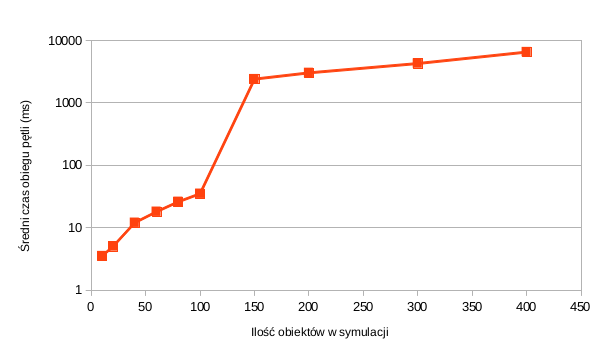
\includegraphics[width=\textwidth,keepaspectratio]{img/wykres_1}
\textit{Wykres 1. Ilość obiektów a średni czas obiegu pętli.}
\end{center}
}

\par{
Na wykresie tym wyraźnie widać, że ilość zapisów w stosunku do ilości obiektów ma charakter liniowy w dwóch przedziałach z wyraźnym przesunięciem w okolicach 120 obiektów. Powodem tego załamania zdaje się być fakt, że przekroczenie przez czas jednego obiegu pętli zadanego jako stała minimalnego czasu przetwarzania, powoduje, że kolejny obieg pętli będzie odpowiadał dłuższemu odcinkowi symulowanego czasu a więc średnio będzie nań przypadało więcej odczytów z kamer (jako, że kamera odczytuje stan okolicy periodycznie). Zależnie od prawdziwości wyżej wspomnianej hipotezy powinna nastąpić w tym miejscu mniej lub bardziej gwałtowna reakcja lawinowa prowadząca do stanu, w którym każda kamera będzie dokonywała odczytu w każdym obiegu pętli - to właśnie obserwujemy jako załamanie na \textit{wykresie 1}.
}
\par{
Ze względu na dualny charakter tej charakterystyki zdecydowano się przenieść ją do celów badań do jej górnej części, by to załamanie - nieistotne z punktu widzenia celu badan - nie zaciemniało obrazu. W związku z tym zdecydowano się obniżć czas między wyzwoleniami każdej z kamer do zera co powoduje, że każda kamera w każdym obiegu pętli wykona zrzut swojego otoczenia, ponieważ spełniony będzie warunek:
}
\par{
\begin{center}
$T_{wyzwolenia kamer} < \Delta T_{kroku}$
\end{center}
}

\section{Wyniki badań}
\par{
W wyniku badań otrzymano rezultaty zaprezentowane w Tablicy 4.3 oraz na Wykresie 2.
}
	Brak zapisu do bazy danych

\par{
\begin{table}[t]
\caption{Ilość obiektów a średni czas pętli, dla $\Delta T_{wyzwolenia kamer} = 0$}
\label{Tabela 1}
\begin{center}
\begin{tabular}{|c|c|c|}
  \hline 
  \textbf{Ilość obiektów} & \textbf{Czas pętli (ms), zapis do bazy} & \textbf{Czas pętli (ms), brak zapisu do bazy}\\
  \hline
10 & 177 & 2 \\
20 & 375 & 2,5 \\
40 & 674 & 3 \\
80 & 1222 & 4 \\
160 & 2629 & 7 \\
320 & 5052 & 13 \\
640 & 10028 & 31 \\
  \hline  
\end{tabular}
\end{center}
\end{table}
}

\begin{center}
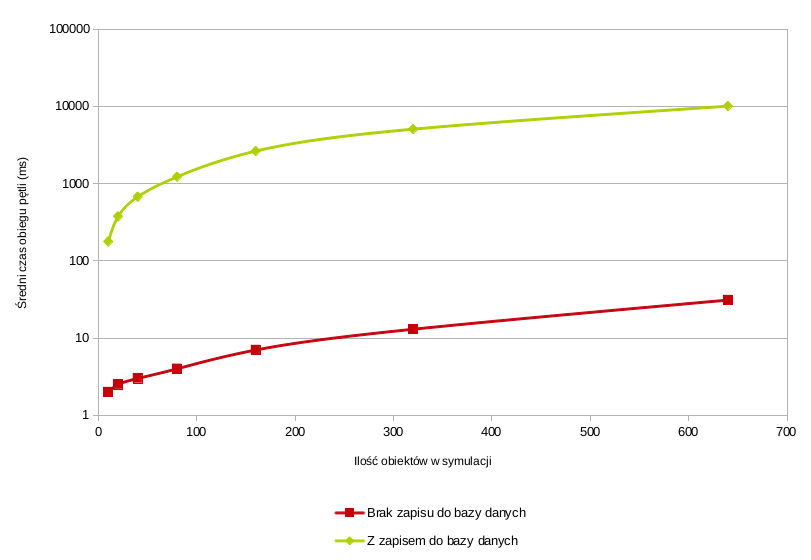
\includegraphics[width=\textwidth,keepaspectratio]{img/wykres_2}
\textit{Wykres 2. Ilość obiektów a średni czas obiegu pętli dla $\Delta T_{wyzwolenia kamer} = 0$.}
\end{center}
}

\par{
Na \textit{wykresie 2} wyraźnie widać, że zarównow przypadku zapisu do bazy danych jak i gdy zapis ten zostanie wyłączony czas trwania pojedyńczego obiegu pętli zależy liniowo od ilości obiektów w symulacji.
}
\par{
Na wykresie w skali logarytmicznej widać też jednak, że w przypadku zapisów do bazy cały wykres przeniesiony jest o rzędy wielkości wyżej - na wykresie w zwykłej skali wariant bez zapisu byłby w ogóle nie widoczny i zredukowany do płaskiego odcinka na dole wykresu.
}
\par{
Wnioskiem z tej obserwacji zdaje się być potwierdzenie hipotezy. W oparciu o proste obliczenia, można natomiast oszacować, że czas operacji wejścia wyjścia to ok. $99.7\%$ całkowitego czasu działania symulacji.
}
\section{Wnioski z badań}
\par{
Ze względu na całkowite zdominowanie czasu pracy symulacji przez czas operacji wejścia-wyjścia optymalizowanie czasu obliczeń na tym etapie prac nie jest racjonalne z punktu widzenia realnego wzrostu wydajności symulacji.
}

\chapter{Podsumowanie}